% file: graph-decomposition/binary-tree-dfs-interval.tex

\documentclass[tikz]{standalone}
\usepackage{tikz-qtree}

\begin{document}
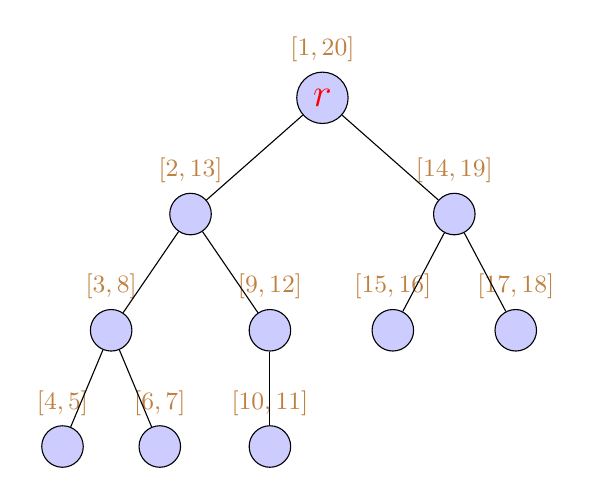
\begin{tikzpicture} [level distance = 42pt, sibling distance = 10pt,
  edge from parent/.style= { % added code
      draw, edge from parent path = {(\tikzparentnode) -- (\tikzchildnode)}}]
  \tikzset{every tree node/.style = 
    {align = center, circle, draw, fill = blue!20, font = \Large, minimum size = 15pt},
    every label/.style = {font = \small, brown}}
    \Tree [.\node [label = {above: $[1,20]$}] {\textcolor{red}{$r$}};
	    [.\node [label = {above: $[2,13]$}] {};
	       [.\node [label = {above : $[3,8]$}] {};
		 \node [label = {above : $[4,5]$}] {};
		 \node [label = {above : $[6,7]$}] {};
	       ]
	       [.\node [label = {above : $[9,12]$}] {};
		 \node [label = {above : $[10,11]$}] {};
	       ]
            ]
	    [.\node [label = {above : $[14,19]$}] {};
	      [.\node [label = {above : $[15,16]$}] {};
	      ]
	      \node [label = {above : $[17,18]$}] {};
	   ] 
        ]
\end{tikzpicture}
\end{document}

